\subsection{Scaling the task pool increases performance} \label{sec:results_task_scaling}
Another important factor to scale is the amount of data a model is trained on. For example, \citet{hoffmann2022training} showed that in order to get the most out of scaling a language model, one must scale the amount of training data at the same rate as the number of parameters. In our case, relevant data come from interaction with different tasks, so we examine the effect of scaling the number and complexity of different tasks in the XLand pool.

\paragraph{Scaling size of task pool.}

Here we examine the effect of varying the number of training tasks from which the auto-curriculum can sample. Recall that in XLand, a task is the combination of a world (the physical layout of terrain and objects) and a game (specifying the goal and production rules). We investigate the effects of training on tasks sampled from a small pool of 200M distinct tasks (4,000 worlds $\times$ 50,000 games) compared with a large pool of 25B distinct tasks (50,000 worlds $\times$ 500,000 games). Table \ref{tab:task-scaling} shows the full experimental setup for these comparisons.

Figure \ref{figure:scaling_tasks} shows higher test score for identically sized models on the larger task pool. As in the other scaling experiments, we especially see improved performance on the $20$\textsuperscript{th} percentile. The results are shown for two different sizes of models, with the larger Transformer yielding a larger gap when scaling the size of the task pool. This suggests that the large models are especially prone to overfitting to a smaller task pool.


\begin{figure}[t!]
    \centering
    \begin{subfigure}[b]{0.49\textwidth}
        \centering
        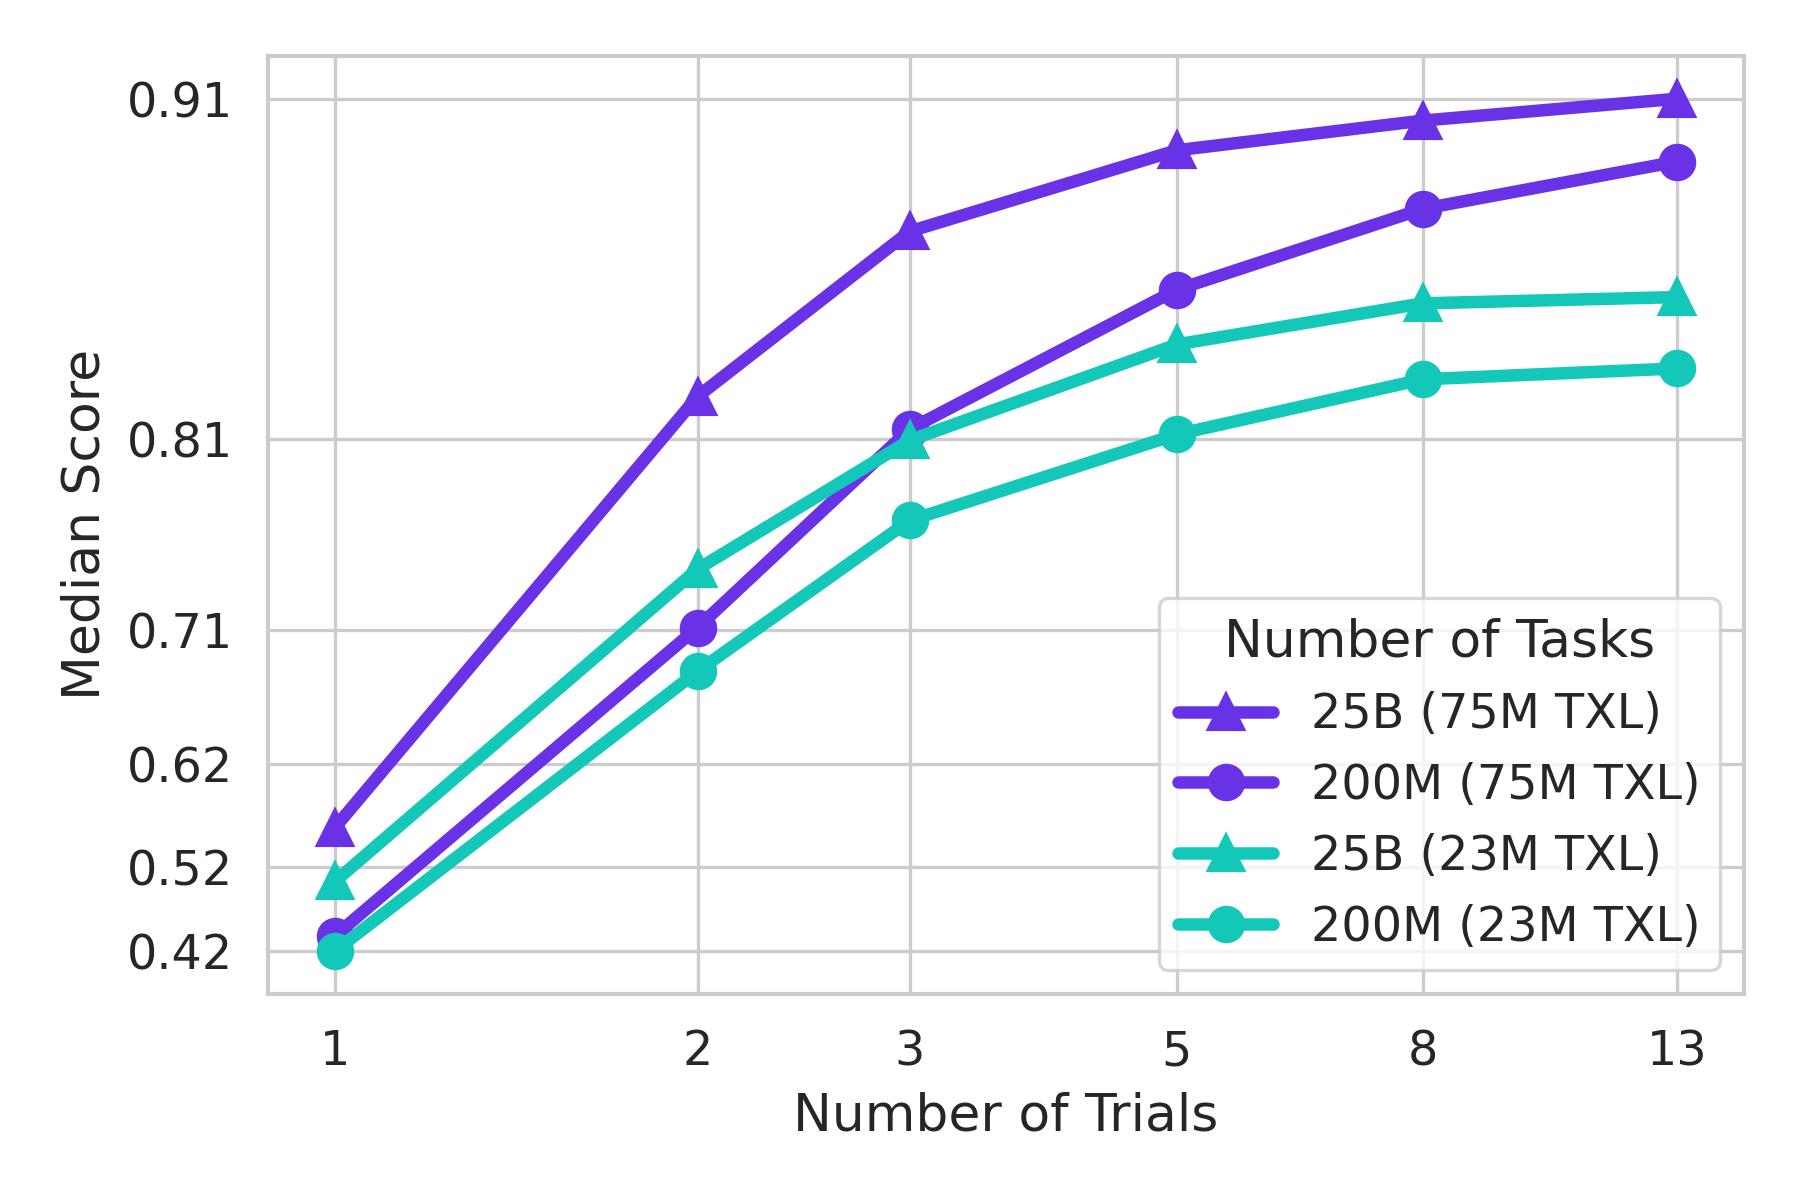
\includegraphics[width=\linewidth]{figures/scaling/task_scaling_25g_steps_percentile50_x_axis_trials_log.png}
        \vskip -3pt \caption{}
    \label{figure:scaling_tasks_50th}
    \end{subfigure}
    \begin{subfigure}[b]{0.49\textwidth}
        \centering
        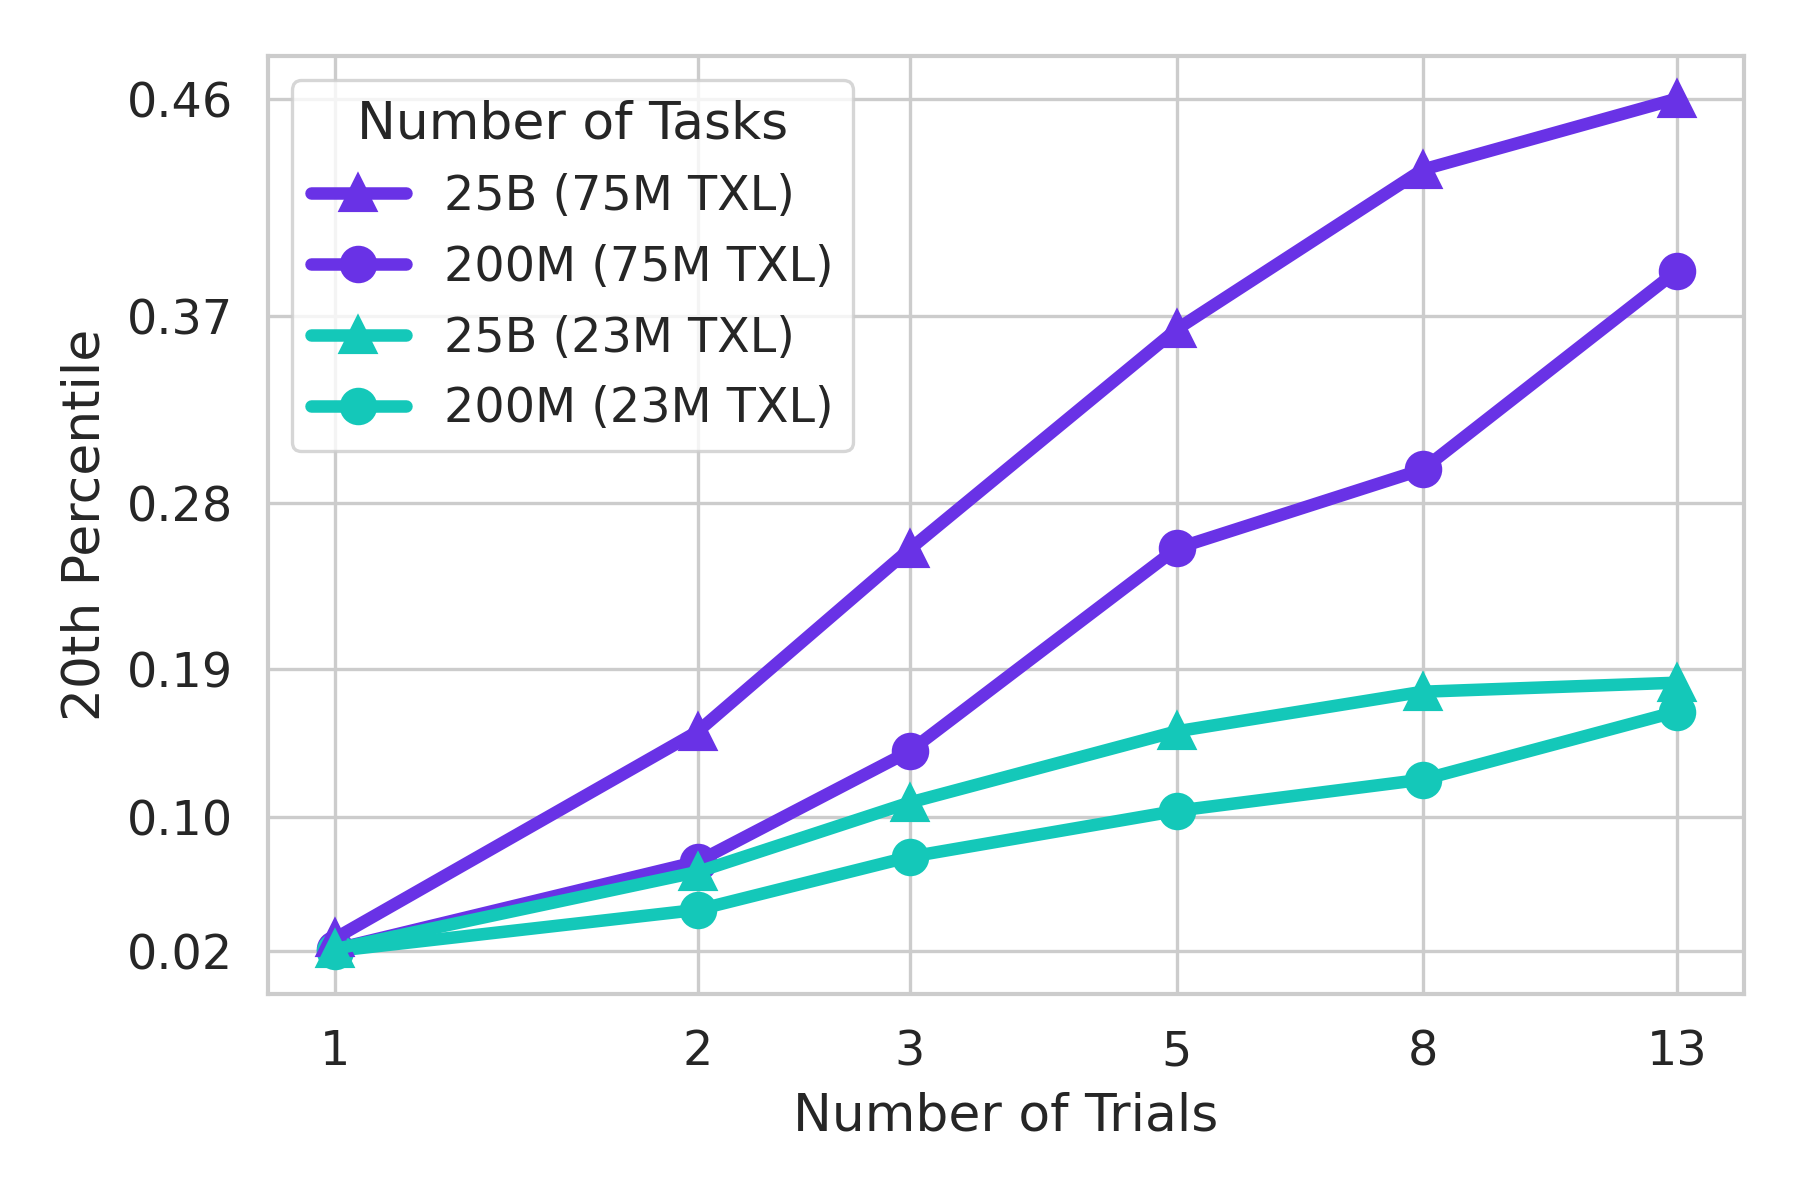
\includegraphics[width=\linewidth]{figures/scaling/task_scaling_25g_steps_percentile20_x_axis_trials_log.png}
        \vskip -3pt \caption{}
    \label{figure:scaling_tasks_20th}
    \end{subfigure}
    \caption{
         Median \textbf{(a)} and 20\textsuperscript{th} percentile \textbf{(b)} adaptation scales with the size of the task pool. The effect is especially prominent for larger models. We show the $y$-axis on a logarithmic scale as in the other scaling experiments. Here, we plot number of trials on the $x$-axis and examine the gaps between the curves for the two task distributions (triangle markers vs. circular markers).
    \label{figure:scaling_tasks}
    }
\end{figure}

\paragraph{Scaling complexity of task pool.}
One final axis along which it is possible to scale our method is the overall complexity of the task distribution. For example, tasks with a flat terrain will be, on average, less complex to solve than tasks with terrain variation. In Figure \ref{app:scaling_complexity}, we show that low environment complexity can be a bottleneck to scaling, by comparing the effectiveness of model scaling between agents trained on two distributions of the same size but different complexity and evaluated on their respective test sets. Open-ended settings with unbounded environment complexity, such as multi-agent systems, may therefore be particularly important for scaling up adaptive agents.